\NeedsTeXFormat{LaTeX2e}
% LTeX: enabled=false
\documentclass[a4paper,
fontsize=12pt,
headsepline,           % Linie zw. Kopfzeile und Text
oneside,               % einseitig
number=noenddot,       % keine Punkte nach den letzten Ziffern in Überschriften
bibliography=totoc,    % LV im IV
%DIV=15,               % Satzspiegel auf 15er Raster, schmalere Ränder   
BCOR=15mm              % Bindekorrektur
%,draft
]{scrbook}
\KOMAoptions{DIV=last} % Neuberechnung Satzspiegel nach Laden von Paket helvet
% \usepackage{scrhack}

\pagestyle{headings}
\usepackage{blindtext}

% für Texte in deutscher Sprache
\usepackage[ngerman]{babel}
\usepackage[utf8]{inputenc}
\usepackage[T1]{fontenc}

% Helvetica als Standard-Dokumentschrift
\usepackage[scaled]{helvet}
\renewcommand{\familydefault}{\sfdefault} 

\usepackage{graphicx}

% be able to include real vector graphics in thesis. You need inkscape installed and your pdflatex command must be called with --shell-escape for this to work.
% TeXstudio: Options → Configure → Commands → pdflatex = pdflatex -synctex=1 -interaction=nonstopmode --shell-escape %.tex
% inkscape=newer to avoid re-export if nothing has changed in the svg. inkscapelatex=false for not using latex to render text (which in turn messes up all text in image). inkscapearea = page so that the SVG size is respected and borders in the SVG are not cut off
\usepackage[inkscape=newer, inkscapelatex=false, inkscapearea=page, inkscapepath=out/_svg]{svg}

% Literaturverzeichnis mit BibLaTeX
\usepackage[babel,german=quotes]{csquotes}
\usepackage[backend=biber]{biblatex}
\addbibresource{MA.bib}
\bibliography{bibliography}

% Alternative mit Paket-Option backend=biber und \addbibresource
% \usepackage[backend=biber]{biblatex}
% \addbibresource{bibliography.bib}

% Für Tabellen mit fester Gesamtbreite und variabler Spaltenbreite
\usepackage{tabularx} 

% Besondere Schriftauszeichnungen
\usepackage{url}              % \url{http://...} in Schreibmaschinenschrift
\usepackage{color}            % zum Setzen farbigen Textes

\usepackage{amssymb, amsmath} % Pakete für Mathe-Umgebungen und -Symbole

\usepackage{setspace}         % Paket für div. Abstände, z.B. ZA
%\onehalfspacing              % nur dann, wenn gefordert; ist sehr groß!!
\setlength{\parindent}{0pt}   % kein linker Einzug der ersten Absatzzeile
\setlength{\parskip}{1.4ex plus 0.35ex minus 0.3ex} % Absatzabstand, leicht variabel

% Tiefe, bis zu der Überschriften in das Inhaltsverzeichnis kommen
\setcounter{tocdepth}{3}      % ist Standard

\usepackage{xcolor} % to access the named colour LightGray
\definecolor{LightGray}{gray}{0.9}

\usepackage[
  outputdir=out,
  ]{minted}
\setminted{
framesep=2mm,
baselinestretch=1.0,
bgcolor=LightGray,
fontsize=\footnotesize
% ,linenos
}
\makeatletter
\ifdefined\minted@optlistcl@quote
\ifwindows
  \renewcommand{\minted@optlistcl@quote}[2]{%
    \ifstrempty{#2}{\detokenize{#1}}{\detokenize{#1="#2"}}}
\else
  \renewcommand{\minted@optlistcl@quote}[2]{%
    \ifstrempty{#2}{\detokenize{#1}}{\detokenize{#1='#2'}}}
\fi
\fi

% similar to \minted@def@optcl@switch
\newcommand{\minted@def@optcl@novalue}[2]{%
  \define@booleankey{minted@opt@g}{#1}%
    {\minted@addto@optlistcl{\minted@optlistcl@g}{#2}{}%
     \@namedef{minted@opt@g:#1}{true}}
    {\@namedef{minted@opt@g:#1}{false}}
  \define@booleankey{minted@opt@g@i}{#1}%
    {\minted@addto@optlistcl{\minted@optlistcl@g@i}{#2}{}%
     \@namedef{minted@opt@g@i:#1}{true}}
    {\@namedef{minted@opt@g@i:#1}{false}}
  \define@booleankey{minted@opt@lang}{#1}%
    {\minted@addto@optlistcl@lang{minted@optlistcl@lang\minted@lang}{#2}{}%
     \@namedef{minted@opt@lang\minted@lang:#1}{true}}
    {\@namedef{minted@opt@lang\minted@lang:#1}{false}}
  \define@booleankey{minted@opt@lang@i}{#1}%
    {\minted@addto@optlistcl@lang{minted@optlistcl@lang\minted@lang @i}{#2}{}%
     \@namedef{minted@opt@lang\minted@lang @i:#1}{true}}
    {\@namedef{minted@opt@lang\minted@lang @i:#1}{false}}
  \define@booleankey{minted@opt@cmd}{#1}%
      {\minted@addto@optlistcl{\minted@optlistcl@cmd}{#2}{}%
        \@namedef{minted@opt@cmd:#1}{true}}
      {\@namedef{minted@opt@cmd:#1}{false}}
}

\minted@def@optcl@novalue{custom lexer}{-x}

\makeatother
\renewcommand{\MintedPygmentize}{./pygmentize.py}


% hier Namen etc. einsetzen
\newcommand{\fullname}{Hannah Lappe}
\newcommand{\email}{hannah.lappe@uni-ulm.de}
\newcommand{\titel}{Case-study for SvelteKit in a Modern Business Application}
\newcommand{\jahr}{2023}
\newcommand{\matnr}{922114}
\newcommand{\gutachterA}{Prof.\,Dr.\,Manfred Reichert}
\newcommand{\gutachterB}{Prof.\,Dr.\,Rüdiger Pryss}
\newcommand{\betreuer}{Dr.\,Marc Schickler\\Jens Scheible}

% hier die Fakultät auswählen
%\newcommand{\fakultaet}{---  Im Quellcode anpassen nicht vergessen! ---}
\newcommand{\fakultaet}{Ingenieurwissenschaften, Informatik und\\Psychologie}
%\newcommand{\fakultaet}{Mathematik und\\Wirtschafts-\\wissenschaften}
%\newcommand{\fakultaet}{Medizin}
%\newcommand{\fakultaet}{Naturwissenschaften}

% hier das Institut einsetzen
\newcommand{\institut}{Institut für Datenbanken und Informationssysteme}

% Informationen, die LaTeX in die PDF-Datei schreibt
\pdfinfo{
  /Author (\fullname)
  /Title (\titel)
  /Producer     (pdfeTex 3.14159-1.30.6-2.2)
  /Keywords ()
}

\usepackage{hyperref}
\hypersetup{
pdftitle=\titel,
pdfauthor=\fullname,
pdfsubject={Masterarbeit},
pdfproducer={pdfeTex 3.14159-1.30.6-2.2},
colorlinks=false,
pdfborder=0 0 0	% keine Box um die Links!
}

% Trennungsregeln
\hyphenation{Sil-ben-trenn-ung}

% LTeX: enabled=true

\begin{document}
\frontmatter

% Titelseite
\thispagestyle{empty}
\begin{addmargin*}[4mm]{-10mm}

  \hfill
  
\includegraphics[height=1.8cm]{assets/logo_uulm_sw.png}\\[1em]

  % LTeX: language=de-DE
  {\footnotesize
  %{\bfseries Universität Ulm} \textbar ~89069 Ulm \textbar ~Germany
  \hspace*{115mm}\parbox[t]{35mm}{\bfseries Fakultät für\\
    \fakultaet\\
    % TODO hier Institut anpassen
    \mdseries \institut}\\[2cm]

  \parbox{140mm}{\bfseries \LARGE \titel}\\[2.5em]
  {\footnotesize Abschlussarbeit an der Universität Ulm}\\[3em]

  {\footnotesize \bfseries Vorgelegt von:}\\
  {\footnotesize \fullname\\ \email}\\ \matnr\\[2em]
  {\footnotesize \bfseries Gutachter:}\\
  {\footnotesize \gutachterA\\ \gutachterB}\\[2em]
  {\footnotesize \bfseries Betreuer:}\\
  {\footnotesize \betreuer}\\\\
  {\footnotesize \jahr}
  }
\end{addmargin*}


% Impressum
\clearpage
\thispagestyle{empty}
{ \small
  \flushleft
  Fassung \today \\\vfill
  \copyright~\jahr~\fullname\\[0.5em]
  % Wenn Sie Ihre Arbeit unter einer freien Lizenz bereitstellen möchten, können Sie die nächste Zeile in Ihren Code aufnehmen. Bitte beachten Sie, dass Sie hierfür an allen Inhalten, inklusive enthaltener Abbildungen, die notwendigen Rechte benötigen! Beim Veröffentlichungsexemplar Ihrer Dissertation achten Sie bitte darauf, dass der Lizenztext nicht den Angaben in den Metadaten der genutzten Publikationsplattform widerspricht. Nähere Information zu den Creative Commons Lizenzen erhalten Sie hier: https://creativecommons.org/licenses/
  %This work is licensed under the Creative Commons Attribution 4.0 International (CC BY 4.0) License. To view a copy of this license, visit \href{https://creativecommons.org/licenses/by/4.0/}{https://creativecommons.org/licenses/by/4.0/} or send a letter to Creative Commons, 543 Howard Street, 5th Floor, San Francisco, California, 94105, USA. \\
  Satz: PDF-\LaTeXe
}

% ab hier Zeilenabstand etwas größer 
\setstretch{1.2}

\tableofcontents

\mainmatter
\chapter{Introduction}
\label{ch:introduction}

Over the past decade, single page applications (SPAs) have become the most popular approach for developing websites. This development was fueled by JavaScript frameworks such as React, Angular and Vue.js which made it easy to develop feature rich web applications. But modern web applications need to satisfy a growing number of technical requirements. Features, such as server side rendering (SSR), code splitting, application routing, and state management have become ubiquitous. This has led to a point where it has become difficult to start new projects from scratch.

To address this issue, in recent years the JavaScript ecosystem saw the emergence of so-called meta frameworks. Meta frameworks are JavaScript libraries that try to fit the role of opinionated "batteries included" frameworks, known from other programming languages, such as Ruby on Rails or Django. They provide out of the box support for many of the features required for building modern web applications. Thus, developers need to spend less time thinking about software architecture and can spend more time thinking about business requirements. Furthermore, meta frameworks can use JavaScript for both frontend and backend, which allows for a tighter integration between the two. Therefore, they can enable a more streamlined development experience, as well as reducing overall application complexity.

SvelteKit is an up-and-coming meta framework that is rapidly gaining popularity. It has multiple advantages over traditional SPA frameworks. SvelteKit allows per page control over the rendering strategy. This allows to render different parts of an application with SSR, client side rendering (CSR) or at build time with pre-rendering. Furthermore, SvelteKit uses various compile time optimizations to produce a more efficient and performant JavaScript bundle. Moreover, it provides functionality, such as reactive state management, component composition, and streamlined data fetching, which helps in writing concise and readable code. Overall, SvelteKit promises to make development of modern web applications faster, while simultaneously improving developer experience.

\section{Problem Statement}
\label{sec:problem-statement}

SvelteKit claims to speed up the development process by handling many common technical requirements of modern web development, but these claims are largely undocumented, furthermore business applications tend to differ in its technical requirements from regular public facing web applications. Thus, it is unclear if SvelteKit would be a good fit for the development of modern business applications

\section{Purpose of this Study}
\label{sec:purpose-of-this-study}
This study provides evidence towards SvelteKit's applicability for the development of modern business applications. To this end we compare two implementations of the same business application in terms of performance, development effort, and code complexity. Furthermore, we provide further considerations when using SvelteKit in production.

In this study, we investigate how SvelteKit's claimed benefits translate to the development of business applications. To this end we reimplement parts of an application that is used to schedule rides for a chauffeur service provided by a federal agency. We compare the resulting application with the original implementation in terms of performance and development effort. Furthermore, we want to generalize the results from this project to typical business applications and try to provide a blueprint for future projects.

% \section{Research Questions}

% Broad research questions: Is SvelteKit a good fit for business applications?
% \begin{enumerate}
%     \item How does performance of SvelteKit compare to other frameworks?
%           \begin{enumerate}
%               \item First contentful paint (FCP)?
%               \item Time to interactive (TTI)?
%               \item Bundle size?
%           \end{enumerate}
%     \item How does SvelteKit improve DX compared to a traditional frontend/backend ?
%           \begin{enumerate}
%               \item Lines of code (LoC)?
%               \item Ecosystem?
%           \end{enumerate}
% \end{enumerate}

\section{Thesis Structure}
\todo{Thesis structure}

% \begin{enumerate}
%     \item Fundamentals
%     \item related work
%     \item implementation
%     \item evaluation
% \end{enumerate}

\chapter{Fundamentals}
\label{ch:fundamentals}

\todo{Chapter introduction}

\todo{Somehow integrate introduction to React Server Components / Next.js}

\section{Enterprise Applications}
\label{sec:enterprise-applications}

% Our applications usually not public facing $\rightarrow$ SEO not relevant $\rightarrow$ SSR, FCP, TTI not as relevant

% - few users up to thousands of users
% - multi-language support
% - stammdatenverwaltung
% - custom framework only relevant for use cases not satisfied by of the shelf software

An enterprise application is software which is used by companies, rather than individual users. Their purpose is to alleviate tasks commonly found in the management and organization process of an enterprise. Common tasks for enterprise applications can be:
\begin{itemize}
    \item enterprise communication
    \item business intelligence (BI)
    \item customer relationship management (CRM)
    \item human resource management (HRM)
    \item enterprise resource planning (ERP)
\end{itemize}

Requirements of an enterprise application can differ vastly depending on its use case, targeted user group, company size, company location, and scope \cite{noauthor_what_nodate,beal_what_2010}. While many ready-made software solutions exist which provide support for common tasks such as ERP, HRM, and CRM, it is often not possible to map all processes of an enterprise to an of-the-shelf component. To this end custom software is often required, which is specifically developed for the given use-case.

\section{Web Development}
\label{sec:web-development}

\subsection{Rendering Patterns}
\label{sec:rendering-patterns}

% \begin{itemize}
%     \item At first only static files
%     \item later SSR (PHP and stuff)
%     \item CSR with dominance of SPA's heralded by React
%     \item now step back to hybrid approach using SSR or SSG with client side hydration.
% \end{itemize}

The rendering of web pages has evolved significantly over the years, with various techniques emerging to enhance user experience. 

\subsubsection{Static HTML}
Static HTML represents the most basic form of web page rendering. In this approach, the entire HTML content is generated on the server and sent to the client as a complete document. Static HTML offers exceptional performance, as there is minimal processing required on the client and server side. However, it lacks dynamic content updates and interactivity, making it suitable primarily for simple, non-interactive websites.

\subsubsection{Server-Side Rendering}
Server-side Rendering (SSR) involves rendering web pages on the server, where both HTML and initial data are generated. The server delivers a fully populated HTML page to the client, improving initial load times and SEO performance. SSR is well-suited for content-heavy and dynamic websites, as it combines good performance with dynamic data capabilities. However, it may still require additional client-side processing for interactive features.

\subsubsection{Client-Side Rendering}
Client-side rendering (CSR) shifts the rendering process to the client's browser. Initially, the server sends a minimal HTML template and JavaScript code. The browser then takes responsibility for rendering and fetching data, making CSR ideal for highly interactive web applications. However, CSR can result in slower initial page load times and worse SEO due to delayed rendering and indexing.

\subsubsection{Static-Site Generation}
Static-site Generation (SSG) is a more extreme form of SSR. Instead of rendering the content when the page is requested, it is instead rendered when the site is initially built. This result in a page with similar performance to static HTML and therefore improved SEO. But, because the page has to be rebuilt, every time content should change, it is only usable for content that rarely changes. This approach can also cause scaling issues in projects with a large amount of different pages. When using SSR these pages could be handled by a dynamic route which fetches the pages content from a headless content management system. With SSG model on the other hand, for each page a separate HTML file is generated during build-time. In extreme cases, this can mean large storage requirements. 

\subsubsection{Hydration}
When server rendered or static web pages are sent to the client side they initially are not interactive beyond the scope of default HTML functionality. Hydration refers to the process of turning this "dumb" web page into a fully interactive client-side Application. With hydration an application can benefit from the fast render times and improved SEO of SSR and SSG, while simultaneously providing the user experience improvements of client-side applications.

\begin{figure}
    \centering
    \begin{sequencediagram}
      \newthread{A}{Client}{}
      \newinst[1]{B}{Server}{}
      \newinst[1]{C}{Database}{}
      \begin{call}{A}{visit /home}{B}{index.html}
      \end{call}
      \begin{call}{A}{request Data}{B}{}
        \begin{call}{B}{SELECT *}{C}{}
        \end{call}
      \end{call}
      \begin{callself}{A}{render data}{}
      \end{callself}
    \end{sequencediagram}

    \label{fig:timing-spa}
    \caption{Example load timing for an application using client-side rendering.}
\end{figure}

\subsection{Meta Frameworks}

\section{Svelte}
\label{sec:svelte}

Svelte was created in 2016 by Rich Harris as a successor to Ractive.js \cite{offerzen_origins_svelte_2022}. It is a framework for developing web user interfaces, similar to React, Angular, and Vue.js. Harris describes Svelte as a framework not to run code but to think about code \cite{offerzen_origins_svelte_2022}. Svelte's key difference compared to other web UI frameworks is, that it uses a Compiler. This makes it possible to shift many rendering steps from the run time into the build time. Therefore, Svelte can ship smaller and more efficient bundles. Furthermore, Svelte's Syntax can do things which would not be possible in vanilla JavaScript.

\subsection{Features}

\todo{Write something here}

\subsubsection{Svelte Files}
% - Files with .svelte ending
% - Syntax very similar to regular html with some extensions
% - standard javascript/Typescript $=>$ existing tools can be more easily integrated
% - javascript/html/css colocated in same file
% - {} to use js expressions in html, similar to react.
% - shorthand attribute syntax

Svelte is a custom language that is very similar to HTML, JavaScript, and CSS, which is colocated inside a \texttt{.svelte} file. In fact, plain HTML syntax is also valid Svelte syntax:

\begin{myminted}{svelte}{app.svelte}
<h1>Hello World!</h1> 
\end{myminted}

Logic can be added with a \texttt{<script>}-block and variables can be used outside the HTML with curly-braces:

\begin{myminted}{svelte}{}
<script>
    const name = 'world';
</script>

<div>Hello {name.toUpperCase()}!</div>
\end{myminted}

Similar to React, variables can also be used in element attributes, and Svelte even provides a shorthand when variable name and attribute name are the same:
\begin{myminted}{svelte}{}
<script>
    const src = './some/img.svg';
</script>

<img src={src}>
<img {src}> 
\end{myminted}

\subsubsection{Reactivity}
% - asignments with usual js asignments. would not work in React.
% - unlike react, svelte runs script just once, for assignments, svelte inserts invalidate blocks to update a variable
% - compare svelte to equivalent react code.

Svelte provides a strong system for reactivity. Mutation of variables is done with regular assignment operations:

\begin{myminted}{svelte}{}
<script>
    let count = 0;

    function increment() {
        count += 1;
    }
</script>

<div>count: {count}!</div>
<button on:click={increment}>click me!</button>
\end{myminted}

This is possible, because Svelte's compiler replaces assignment operations at build time. The increment function in the prior example would be compiled to this statement:

\begin{myminted}[escapeinside=||]{js}{}
function increment() {
    |\$\$|invalidate('count', count += 1)
}
\end{myminted}

An equivalent React implementation using function components would have to use more verbose semantics, because without a specialized compiler, assignment operations do not have any special meaning:

\begin{myminted}{jsx}{}
function Component() {
    const [count, setCount] = useState(0);

    function increment() {
        setCount(c => c + 1);
    }

    return <>
        <div>count: {count}!</div>
        <button onClick={increment}>click me!</button>
    </>
}
\end{myminted}

React's code runs every time, a component is updated, this means derived values can just be declared, and they are evaluated every time. Svelte's code on the other hand, only runs once on component initialization. Therefore, Svelte introduces custom syntax for defining reactive statements. To This end, Svelte repurposes labeled statements:


\begin{myminted}[highlightlines={4},escapeinside=||]{svelte}{}
<script>
    let count = 2;

    |\$|: doubled = count * 2;

    function increment() {
        count += 1;
    }
</script>

<button on:click="{increment}">click me!</button>
<div>count: {count}!</div>
<div>doubled: {doubled}!</div>
\end{myminted}

% - $: to make reactive statement
% - repurpose of rarely used js feature
% - used for reactive assignments, conditions, and whole codeblocks
% - reactive block is rerun everytime a variable used inside the block changes

\mintinline{js}{$:} marks a statement as reactive. Every time a value, that is used in a reactive statement, changes, the statement is reevaluated. This can be used for assignments, as seen in the prior example, but it can also be used for conditions and code blocks:

\begin{myminted}[escapeinside=||]{svelte}{}
<script>
    let count = 0;

    |\$|: {
        console.log(`new value of count: ${count}`);
        console.log('This will also be executed when count changes');
    }

    |\$|: if(count > 9) {
        console.log('It is over 9!');
        count = 0;
    }
</script>
\end{myminted}
\s{$}

\subsubsection{Templates}

% - Templates for if, each

HTML does not have a way of expressing logic, thus Svelte introduces its own syntax. To conditionally render some markup, it is wrapped inside an if-block:

\begin{myminted}[highlightlines={11-14}]{svelte}{}
<script>
    let count = 0;

    function increment() {
        count += 1;
    }
</script>

<button on:click={increment}>click me!</button>
<div>count: {count}!</div>
{#if count > 9}
    <div>Vegeta what does the scouter say about his power level?</div>
    <div>It's over 9!!</div>
{:else}
    <div>The number ir pretty low</div>
{/if}
\end{myminted}

UI's also often work with lists of data. To this end, Svelte provides an each-block, which can be used to handle repeating data:

\begin{myminted}[highlightlines={5-7}]{svelte}{}
<script>
    let array = [1, 2, 3, 4];
</script>

{#each array as value}
    <div>{value}</div>
{/each}
\end{myminted}

\subsubsection{Components}

% - Since emergence of React, component driven development became norm.
% - in Svelte, one file = one component.
% - Name = Component Name.

% todo: citation needed
Since the emergence of React in 2013, component-driven user-interfaces have become a widespread approach to web development. In Svelte, a component is represented by a singular \mintinline{html}|.svelte|-file, where the file name determines the component name: 

\begin{myminted}{html}{MyComponent.svelte}
<script>
    export let value;
</script>

<div>hello, {value}!</div>
\end{myminted}

To define props on a Component, Svelte repurposes the \mintinline{js}|export| keyword. The Component can than be imported and used like a regular element:

\begin{myminted}{svelte}{app.svelte}
<script>
    import MyComponent from './MyComponent.svelte';

    let value = 'world';
</script>

<MyComponent {value} />
\end{myminted}

\subsubsection{Events}

% - possible to listen to any event with on: 
% - custom events also

In a prior example we already showed usage of \mintinline{svelte}|on:click|. This directive is used to listen to click events. Svelte make sit possible to listen for arbitrary events on an element with the \mintinline{html}|on|-keyword:

\begin{myminted}[highlightlines={7}]{html}{}
<script>
    function handleMove(event) {
        // ...
    }
</script>

<div on:pointermove="{handleMove}" ></div>
\end{myminted}

Furthermore, Svelte provides an event dispatcher, so that components can throw their own custom events:

\begin{myminted}{html}{}
<script>
    import { createEventDispatcher } from 'svelte';

    const dispatch = createEventDispatcher();

    function sayHello() {
        dispatch('message', {
            text: 'Hello!'
        });
    }
</script>
\end{myminted}

\subsubsection{Bindings}

% - usually data passed down. Parent can set props of child but not otherway around.
% - Svelte provides tool to work around that
% - simpler compared to react

\begin{myminted}{svelte}{}
<script>
    let name = 'Peter';
</script>

<input bind:value={name} />
\end{myminted}

\begin{myminted}{jsx}{}
function Component() {
    const [name, setName] = useState('Peter');

    return ( 
        <input 
            value={name}
            onChange={e => setName(e.currentTarget.value)} 
        />
    )
}
\end{myminted}

\subsubsection{TypeScript}

Svelte has out of the box support for TypeScript. TypeScript can be enabled for a svelte-file by annotating the  script block with a \mintinline{bash}|lang| attribute:

\begin{myminted}{svelte}{}
<script lang="ts">
    let value: string = "World"
</script>
\end{myminted}

This however, comes with certain restrictions. It is not possible to use TypeScript syntax outside the script block. One might for example want to type the parameters of an inline event handler:

\begin{myminted}{svelte}{}
<input on:change={(e: InputEvent) => {}}> /* this will not work */ 
\end{myminted}

\section{SvelteKit}
\label{sec:sveltekit}

SvelteKit is a framework that builds around Svelte to provide a toolkit for rapidly developing web applications \cite{noauthor_sveltekit_nodate}. It can be used out of the box to develop full stack applications, server rendered frontend applications, static web pages, and traditional single page applications without any server rendering. It provides multiple basic, as well as advanced features, required for the development of modern web applications. Features include routing, support for different rendering patterns, build optimization, data preloading, and zero-configuration deployments. Furthermore, SvelteKit uses Vite\footnote{https://vitejs.dev/} to enable a good development experience, with fast startup times and quick hot module replacement.

In the following we give an overview of multiple SvelteKit concepts and features, that will be relevant for the rest of this study. 

% Meta Framework
% Stable release 2022
% provides functionality for modern applications
% Deployable as static files, web server, edge functions

\subsection{Features}

\todo{Write something here}

\subsubsection{Routing}
\label{sec:sveltekit-routing}

SvelteKit provides out-of-the-box support for Routing. To this end, SvelteKit utilizes a file-system-based routing system. This means that the URL's that a user can access on the web application, directly maps to the directory structure in the project's file system. A SvelteKit project contains a \mintinline{bash}|routes|-directory. This directory marks the root of the URL, e.g.: \mintinline{bash}|http://example.com/|. Respectively, the directory structure \mintinline{bash}|routes/about| would map to \mintinline{bash}|http://example.com/about|. This system ca also be used to create parameterized routes. The directory structure \mintinline{bash}|routes/blog/[slug]| would create a route, where \mintinline{bash}|slug| serves as a wildcard (e.g.: \mintinline{bash}|/blog/hello-world|, \mintinline{bash}|/blog/123|).

The actual content of a page is defined in a \mintinline{bash}|+page.svelte| file:
\begin{myminted}{svelte}{routes/+page.svelte}
<h1>My Website</h1>
<p>Welcome to my website...</p>
\end{myminted}
\begin{myminted}{svelte}{routes/about/+page.svelte}
<h1>About</h1>
<p>about this site...</p>
<a href="/home">Home</a>
\end{myminted}

SvelteKit uses the HTML \mintinline{svelte}|<a>|-tag to navigate between pages, rather than a framework specific \mintinline{svelte}|<Link>|-component. This has the advantage of being progressively enhanceable. If JavaScript is not available on the client-side, the anchor-tag's navigation event can be handled by the browser, and the browser will do a regular full page reload to reach the navigation target. In the case of JS being available, SvelteKit's runtime router will intercept the navigation event and perform an in-app navigation to the target, without causing a full page reload.

Most websites have some elements that should be displayed across multiple pages, such as a navigation bar or a footer. To this end, SvelteKit's router has the concept of layouts. A layout is placed alongside the pages inside the \mintinline{bash}|routes|-directory, inside a \mintinline{bash}|+layout.svelte|-file. This layout will automatically be applied to all route and all sub-routes of the directory, where the layout-file is placed. The place where the actual page content should be rendered inside the layout is defined by a \mintinline{svelte}|<slot>|-element:

\begin{myminted}{svelte}{routes/+layout.svelte}
<nav>
    <a href="/home">home</a>
    <a href="/blog">blog</a>
    <a href="/about">about</a>
</nav>

<slot/>
\end{myminted}

In some cases an application may have multiple routes, that should live on the same route as others, but should have their own shared layout. One could for example imaging a website, where the user authentication pages should have a different layout than the authenticated area of the app. Therefore, SvelteKit provides a mechanism to group routes together without this route being reflected in the URL by wrapping the group name in parentheses:
\begin{myminted}[highlightlines={2,6}]{bash}{}
routes/
  (app)/
    dashboard/
    details/
    +layout.svelte
  (auth)/
    signin/
    register/
    +layout.svelte
\end{myminted}

\subsubsection{Loading Data}
\label{sec:sveltekit-loading}

SvelteKit facilitates a standard way for fetching dynamic content that is to be rendered on a page. This is required to enable SSR and SSG. To this end, every page can have a dedicated load function, that is defined in a \mintinline{bash}|+page.js|-file. When a user requests a page, this load function is executed, and the returned data is passed to the \mintinline{bash}|+page.svelte|-file:

\begin{myminted}{js}{routes/+page.js}
export async function load() {
    const todos = (await fetch('/api/todos')).json();

    return { todos };
}
\end{myminted}
\begin{myminted}{svelte}{routes/+page.svelte}
<script>
    export let data;
</script>

{#each data.todos as todo}
    <div>{todo.name}</div>
{/each}
\end{myminted} 

In SSR mode, when a user first requests a page, the load function is executed on the server. Afterwards the Svelte-file is rendered once, before being sent to the user as populated HTML. In the browser, SvelteKit then hydrates the page. During hydration, SvelteKit runs the load function a second time on the client to create a consistent data model. 

After the app has finished hydrating, all following navigation events will be handled by SvelteKit's runtime router. When the user now navigates to a different page the load function now is invoked on the client-side directly, therefore saving an unnecessary roundtrip to the server. Because these load functions run on both server and the client, they are called universal load functions.

Some data fetching can only take place on the server-side, for example database access. Therefore, SvelteKit also provides a second form of load function, that is only executed on the server. These server load function are placed in \mintinline{bash}|+page.server.js|-files:

\begin{myminted}{js}{routes/+page.server.js}
import db from '$lib/server/db';

export async function load() {
    const todos = await db.getTodos();

    return { todos };
}
\end{myminted}
\s{$}

In the same way as universal load functions, server load functions are executed on the server when a user initially requests a page. But, because they can only run on the server, when a user navigates inside the app, instead of running the load function client-side, the client sends a request to the server for new data. The server then executes the load function and sends the resulting data back to the frontend as JSON. 

This behavior also highlights another difference between universal and server load functions. Because server load functions need to be able to send JSON to the client, all data they return must be serializable. This restriction does not apply to universal load functions. Therefore, they can return arbitrary data such as class instances:

\begin{myminted}{js}{routes/+page.js}
export async function load() {
    const todos =  [ new Todo(`finish master's thesis`) ]

    return { todos };
}
\end{myminted}

\subsubsection{Form Actions}
\label{sec:sveltekit-server-actions}

The previous section discussed how SvelteKit applications send dynamic data to the client. But, many applications also need a way to send data to the server. To this end, SvelteKit provides Form actions. \mintinline{bash}|+page.server.js|-files can export actions, which make it possible to post data to the server using HTML's \mintinline{svelte}|<form>|-elements.

\begin{myminted}{svelte}{routes/+page.server.js}
export const actions = {
    postTodo: async () => {
        // post Todo
    }
}
\end{myminted}    
\begin{myminted}{svelte}{routes/+page.svelte}
<form method="POST" action="?/postTodo">
    <label>
        Todo name:
        <input name="todoName">
    </label>
</form>
\end{myminted}

The name of the action, the form should post to, is specified as a query parameter. This makes it possible to have multiple actions per route. Because the implementation, uses only default HTML forms, it is again possible to progressively enhance this feature. In Fact, in the shown implementation, submitting, would cause a full page reload, because the browser is sending post request to the server. To progressively enhance this form, one can add the \mintinline{bash}|enhance| action:

\begin{myminted}{svelte}{routes/+page.svelte}
<script>
    import { enhance } from '$app/forms';
</script>

<form method="POST" action="?/postTodo" use:enhance>
\end{myminted}  
\s{$}

This action intercepts form submit events and instead posts them to the server as an asynchronous request. This way the UI can provide better user experience, by foregoing the full page refresh. 
 
\subsubsection{Rendering}

SvelteKit provides the functionality to define the rendering strategy for each route independently.
By exporting the constants \mintinline{bash}|ssr|, \mintinline{bash}|csr| and \mintinline{bash}|prerender| the rendering behavior of page can be precisely changed:
\begin{myminted}{js}{routes/page.js}
export const prerender = false;
export const ssr = true;
export const csr = true;
\end{myminted}

\begin{itemize}
    \item Setting \mintinline{bash}|prerender| to true, the page will render this page during the build process and serve this route as static files. This also means this route cannot have form actions, because SvelteKit will not provide handlers for a pre-rendered route.
    \item \mintinline{bash}|ssr| determines if the page should be rendered on the server site when the user first requests the page. This does not mean the page cannot specify a server load function. Instead, the client will simply request the data from the server load function as soon as the runtime is initialized on the client side. This option can sometimes be useful, when a page requires certain features that require access to browser exclusive API's to render its content. But, most of the time it is possible to defer access to these browser-specific API's by running the code after the function has been mounted. 
    \item With \mintinline{bash}|csr| it is possible to completely disable client-side JavaScript. But this has certain side effects. For example, given an application has a layout that contains a navigation bar which needs JavaScript to work. If the user first loads the website on a page that has CSR disabled, the navigation bar will not work. On the other hand, if the user loads the website on a page that has CSR enabled and then navigates to a page with CSR set to false, the navigation bar will work. 
\end{itemize}

\section{UI5}
UI5 is a JavaScript-based web frontend-framework. It Was Developed by SAP, a German enterprise software company. The framework was first open-sourced in 2013 under the title OpenUI5 \cite{kurz_brief_2020}. It is focused on development of enterprise-ready applications. UI5's main selling points are a wide range of integrated features, such as data-bindings, OData-API\footnote{\url{https://www.odata.org/}} support, and localization. Furthermore, UI5 provides many ready-made UI-Components with support for accessibility, keyboard navigation and right-to-left languages \cite{kunz_what_2013}.   

UI5's UI-Components are tightly integrated with Fiori\footnote{\url{https://experience.sap.com/fiori-design/}} a set of UI design guidelines that is optimized for the development of enterprise applications.

\begin{figure}
  \begin{myminted}{xml}{App.view.xml}
    <blub/>
  \end{myminted}
  \begin{myminted}{js}{App.controller.js}
    sap.m.define([], () => {

    })
  \end{myminted}
  \caption{Example of a Component in UI5}
  \label{fig:ui5-mvc}
\end{figure}

\section{Methodology}
\label{sec:methodology}

% This thesis follows the principles of an explorative case study as defined by P. Runeson and M. Höst\cite{runeson_guidelines_2009}. The Authors describe the Process as consisting of five steps:

% \begin{enumerate}
%     \item Case study Design: Objectives are defined, and the case study is planned.
%     \item Preparation for data collection: procedures and protocols for data collection are defined.
%     \item Collecting evidence: execution with data collection on the studied case.
%     \item Analysis of the collected data.
%     \item Reporting
% \end{enumerate}

% As defined in \Cref{sec:purpose-of-this-study}, this study intents to provide evidence that points towards or against SvelteKit's applicability for the development of business applications.

% \subsection{Definition of Data Collection}
% \begin{enumerate}
%     \item Performance metrics
%     \item complexity metrics
% \end{enumerate}

% \subsection{Collection of evidence}

% Metrics applied to all implementations

As defined in \Cref{sec:problem-statement} it is unclear if SvelteKit's claimed benefits translate to the development of real-world applications. To this end, this Study tries to provide evidence that validates SvelteKit's claims. Furthermore, we tried to identify potential shortcomings in SvelteKit's design and feature set. We aim to create a knowledge base of SvelteKit's advantages ad disadvantages which can be used for future technology  choices.

Our primary methodology for achieving this goal involved gaining insights into how SvelteKit behaves in a real-world software project. Therefore, we decided to write an implementation for a real-world use-case existing in an enterprise in the industry. To this end, a project that already has an implementation, which is used in production, was chosen. This has two advantages. Firstly, this makes sure the chosen project is representative for a real-world scenario. Secondly, the existing implementation could serve as a comparison to the created SvelteKit implementation.

The chosen project had to satisfy multiple requirements:
\begin{itemize}
    \item It should have a component responsible for management of datasets.
    \item The application should require authentication.
    \item It should require database persistence.
    \item It should require communication with other services.  
    \item Furthermore, it should have at least one feature that goes beyond basic management of data.
\end{itemize}
These requirements where chosen to make sure the use-case is representative for a wide array of business applications. 

\subsection{Evaluation}
\todo{Explain evaluation process}

Factual evaluation:
\begin{enumerate}
    \item LoC
    \item performance
    \item ecosystem size
\end{enumerate}
\chapter{Related Work}

Because of Svelte's relative novelty, not much scientific work has been published about the language. Nonetheless, we found two works comparing Svelte to other contemporary JavaScript frameworks.

\subsection{Angular and Svelte Frameworks: a Comparative Analysis}

\subsection{DOM benchmark comparison of the front-end JavaScript frameworks React, Angular, Vue, and Svelte}

\begin{itemize}
    \item Levlin\cite{levlin_dom_2020}
    \item comparative performance analysis between, React, Angular, Vue, Svelte.
    \item Performance key takeaway. React, Vue and Angular, Svelte, behave similar because of (not) using virtual DOM.
    \item React winner for mass updates, svelte winner for single updates
    \item BUT, benchmark for mass updates seem disingenuous, because Svelte benchmark does not use Svelte feature and instead directly manipulates DOM. 
\end{itemize}

\subsection{State of JavaScript}

\begin{itemize}
    \item \cite{noauthor_state_nodate}
\end{itemize}
\chapter{Implementation}
\label{ch:implementation}

\todo{Write chapter introduction}

\section{Chauffeur Service}

%  \begin{itemize}
%     \item Take some Pictures
%     \item Chauffeur service for German federal agency.
%     \item Takes new Chauffeur Jobs
%     \item UI overview of Jobs, and Jobs Details
%     \item Overview of Chauffeurs and their availability 
%     \item UI to manage Jobs, assign chauffeurs
%     \item group Jobs
%  \end{itemize}

As a basis for our case study we used an application called DSW-FD (Dispositions-software-Fahrdienst). DSW-FD is used to schedule chauffeur rides for a German federal agency. The application provides a rich user interface with views for managing chauffeur jobs, as well as chauffeur drivers. Clients which need a Chauffeur ride can call a separate hotline, where a handler creates a new chauffeur job, this job is then sent to DSW-FD where it appears in the overview of Jobs and can then be processed by a Job handler.

Drivers need to be manually assigned to a job by a handling person. To this end, the application provides suggestions for drivers which would be free when the job is schedule and are closest to the job's departure point. Furthermore, the app provides functionality to group together different jobs so that they may be handled by a single driver, determine the return destination for the driver after they finished the job, as well as marking a job as being handled by a pool of drivers.

The application also provides features to directly interact with drivers, such as broadcasting messages to all drivers, reminding a driver to take their mandatory break, and directly calling a driver.

\section{Current Implementation}

% \begin{itemize}
%     \item UI5-Frontend
%     \item Java-Backend
%     \item Android app for drivers.
%     \item OIDC
%     \item mssql
% \end{itemize}

The current Implementation is realized as a classic frontend, backend architecture. The backend is implemented using the Java web framework Spring\footnote{\url{https://spring.io/}}. It provides a SOAP web server on which new Jobs are submitted from another service. Data is persisted in a MSSQL database. The backend also provides Multiple REST API's and an OData API for communication with the frontend. Furthermore, the backend has to interact with Firebase to trigger push notifications on smartphone devices.

The System provides two frontends, an android application, which is used by the chauffeur drivers to receive jobs and communication from headquarters and a web client which is used by handlers to manage jobs and drivers. The web client is implemented using OpenUI5\footnote{\url{https://openui5.org/}}. OpenUI5 is a frontend framework published by SAP, it is intended for development of enterprise applications which follow SAP's Fiori design guidelines\footnote{\url{https://experience.sap.com/fiori-design/}}. All APIs of the backend require authentication. To this end the frontend has to authenticate with a Keycloak\footnote{\url{https://www.keycloak.org/}} instance using OpenID Connect (OIDC). An overview of the system architecture is provided in \Cref{fig:dswfd-architecture}.

\begin{figure}[ht]
    \centering
    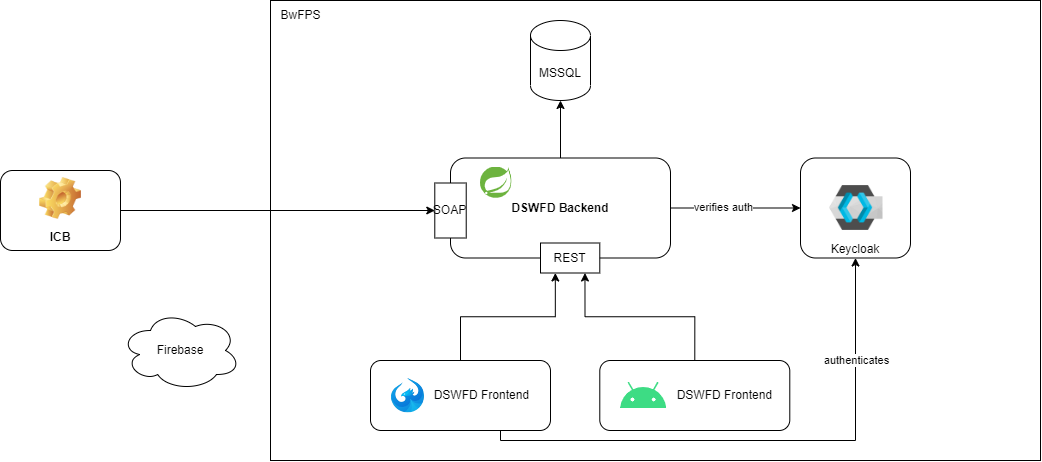
\includegraphics[width=.8\linewidth]{assets/dswfd-architecture}
    \caption{Architecture overview of the current implementation}
    \label{fig:dswfd-architecture}
\end{figure}

\section{SvelteKit Implementation}

% \begin{itemize}
%     \item Two approaches (full stack, FE only)
%     \item First try UI5 web components, second try CSS classes
%     \item Authentication
% \end{itemize}

Our study focused on the core of DSW-FD's system landscape, comprised of the Spring backend and the OpenUI5 web frontend. We experimented with two different implementations. One where SvelteKit replaces both the backend and frontend and one where SvelteKit only replaces the frontend. Both our implementations had to communicate with the Keycloak service to authenticate. The full stack implementation also had to interact with the MSSQL database. As to not widen the scope too much, API's for the android application, Firebase communication, and the SOAP API for ICB was not implemented. We also decided to use TypeScript instead of regular JavaScript. This provided a better developer experience with little extra overhead. Because SvelteKit can infer types for most of its internal functionality. Extra types had to be only defined for external API's.

We focused our implementation on a subset of features required to manage chauffeur jobs. To this end we implemented three pages. The overview page that shows all currently relevant chauffeur jobs (\Cref{fig:current-overview-auftrag}). The detail page for chauffeur jobs (\Cref{fig:current-details-auftrag}). And a view that is used to create new (internal) chauffeur jobs.

\begin{figure}
    \centering
    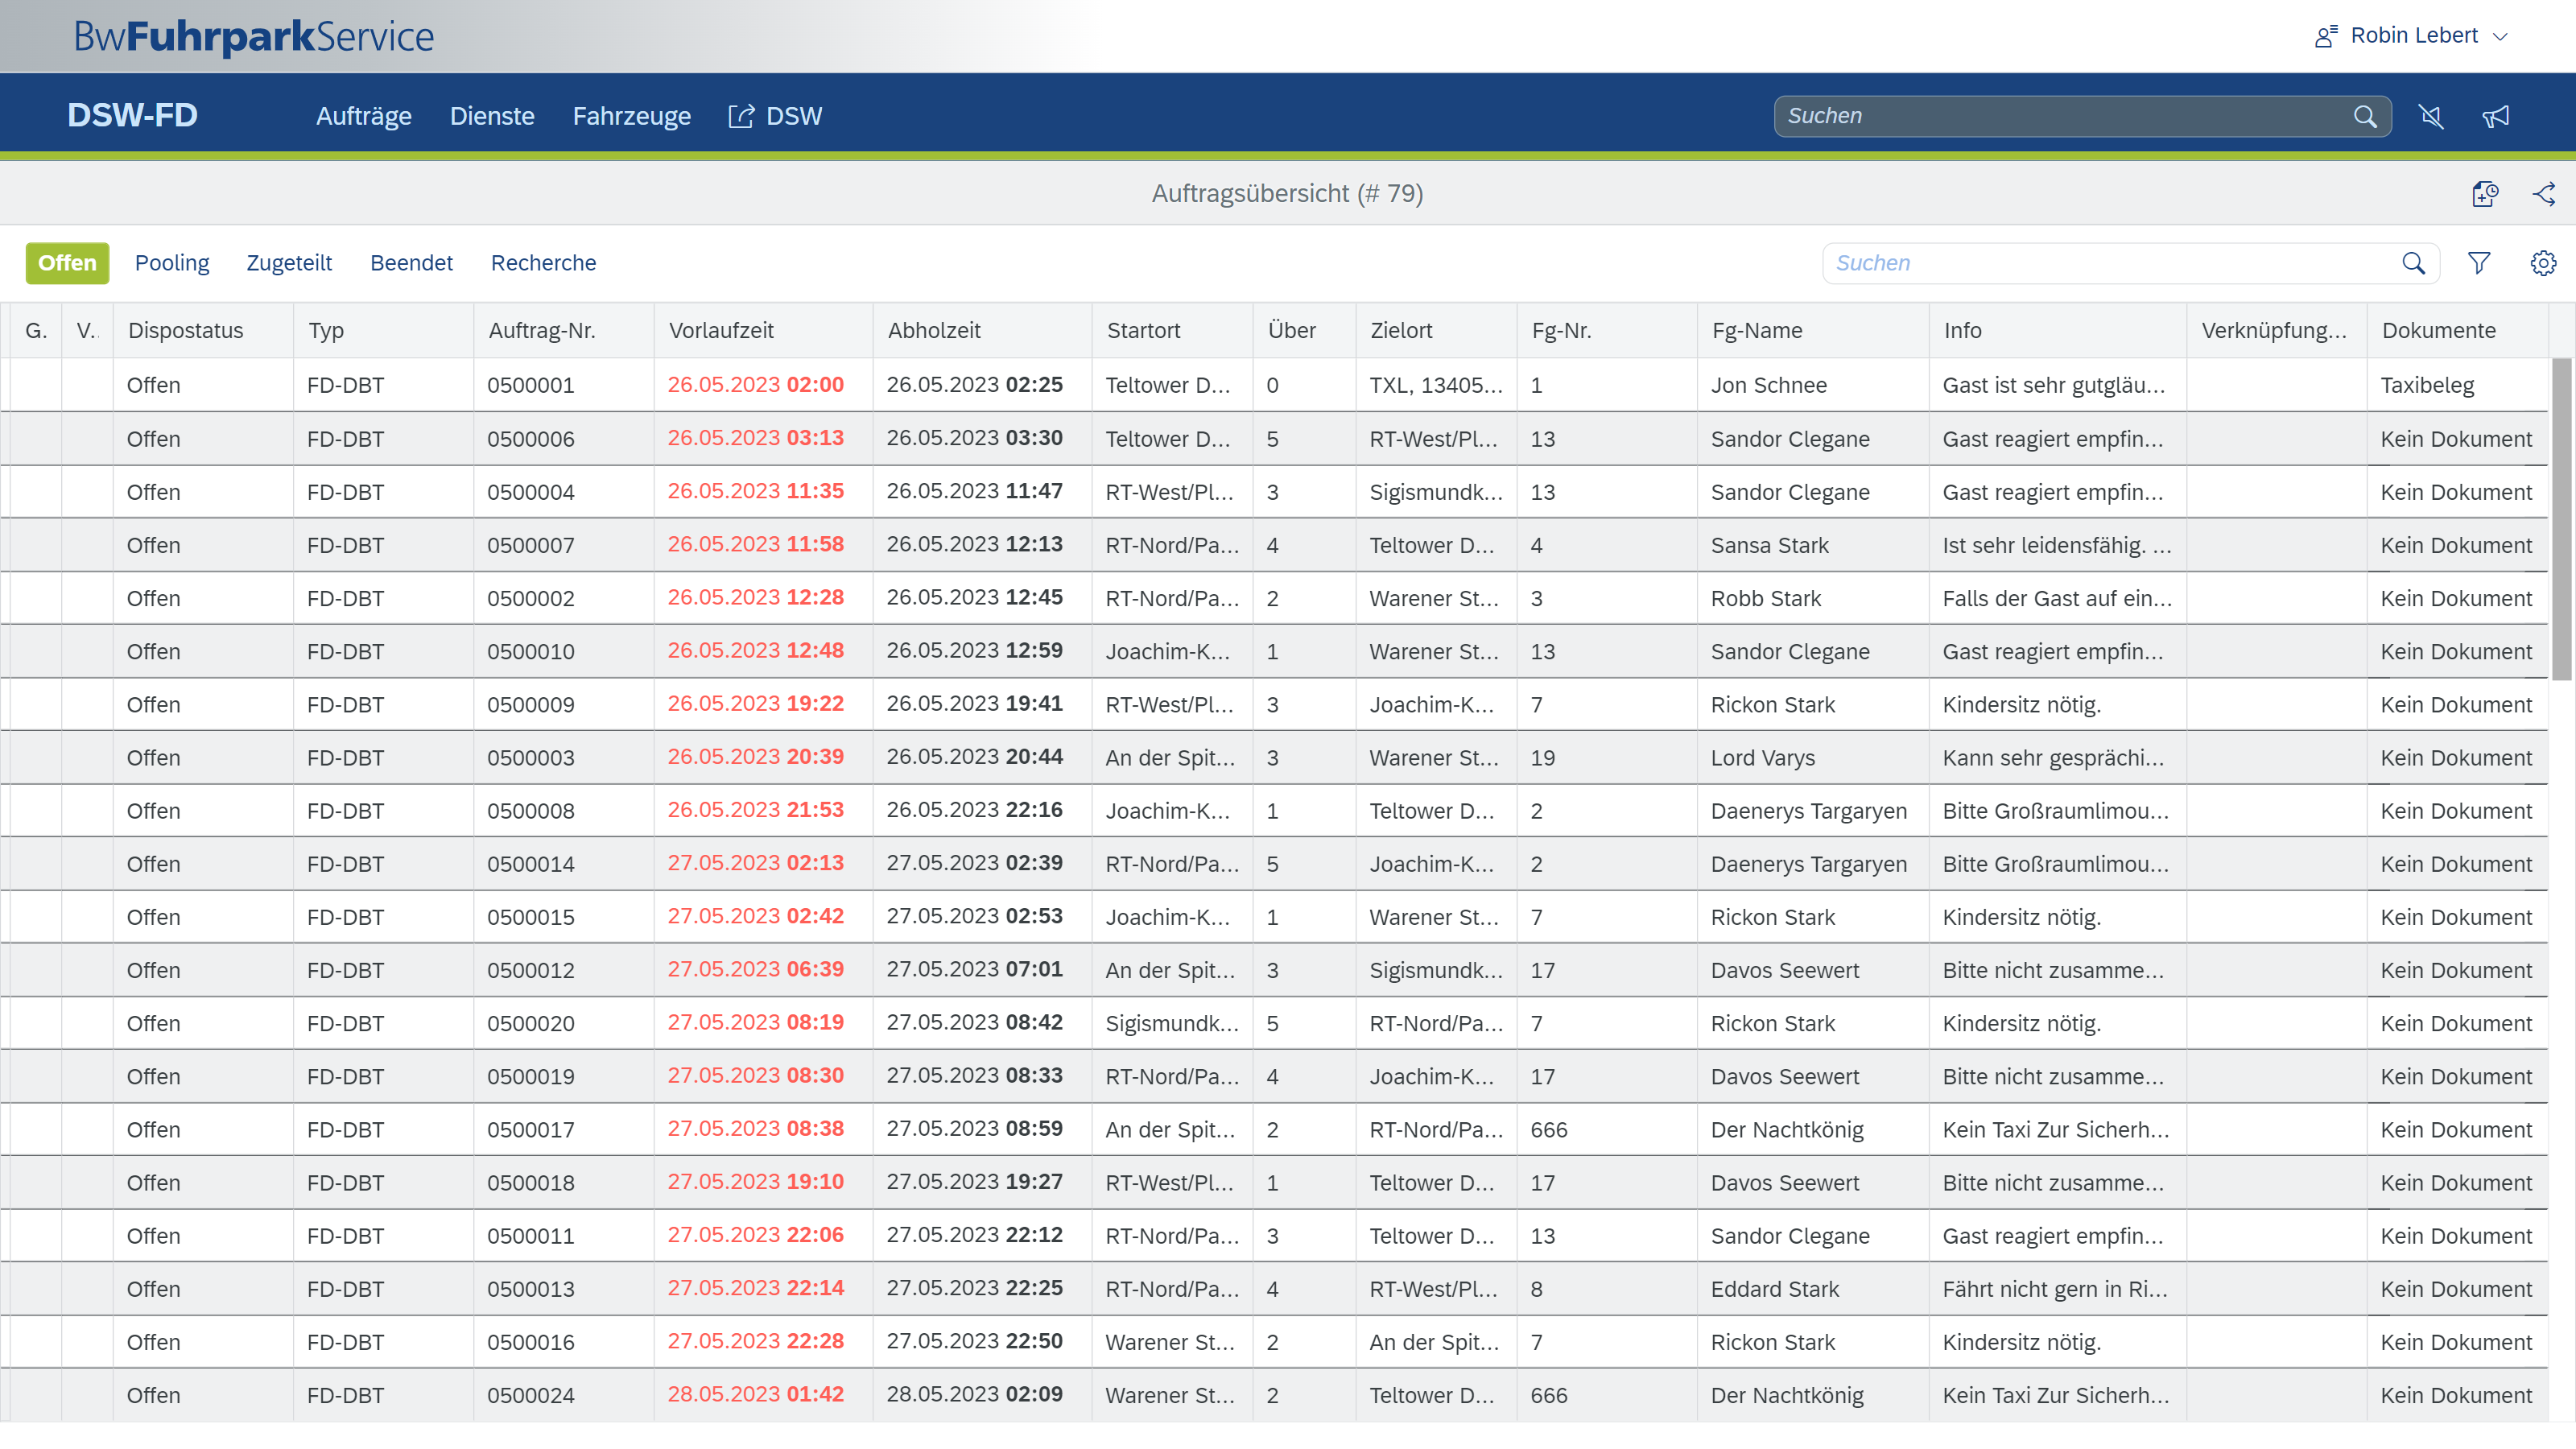
\includegraphics[width=\linewidth]{assets/current-auftrag-overview}
    \caption{Overview of chauffeur jobs in current implementation}
    \label{fig:current-overview-auftrag}
\end{figure}

\begin{figure}
    \centering
    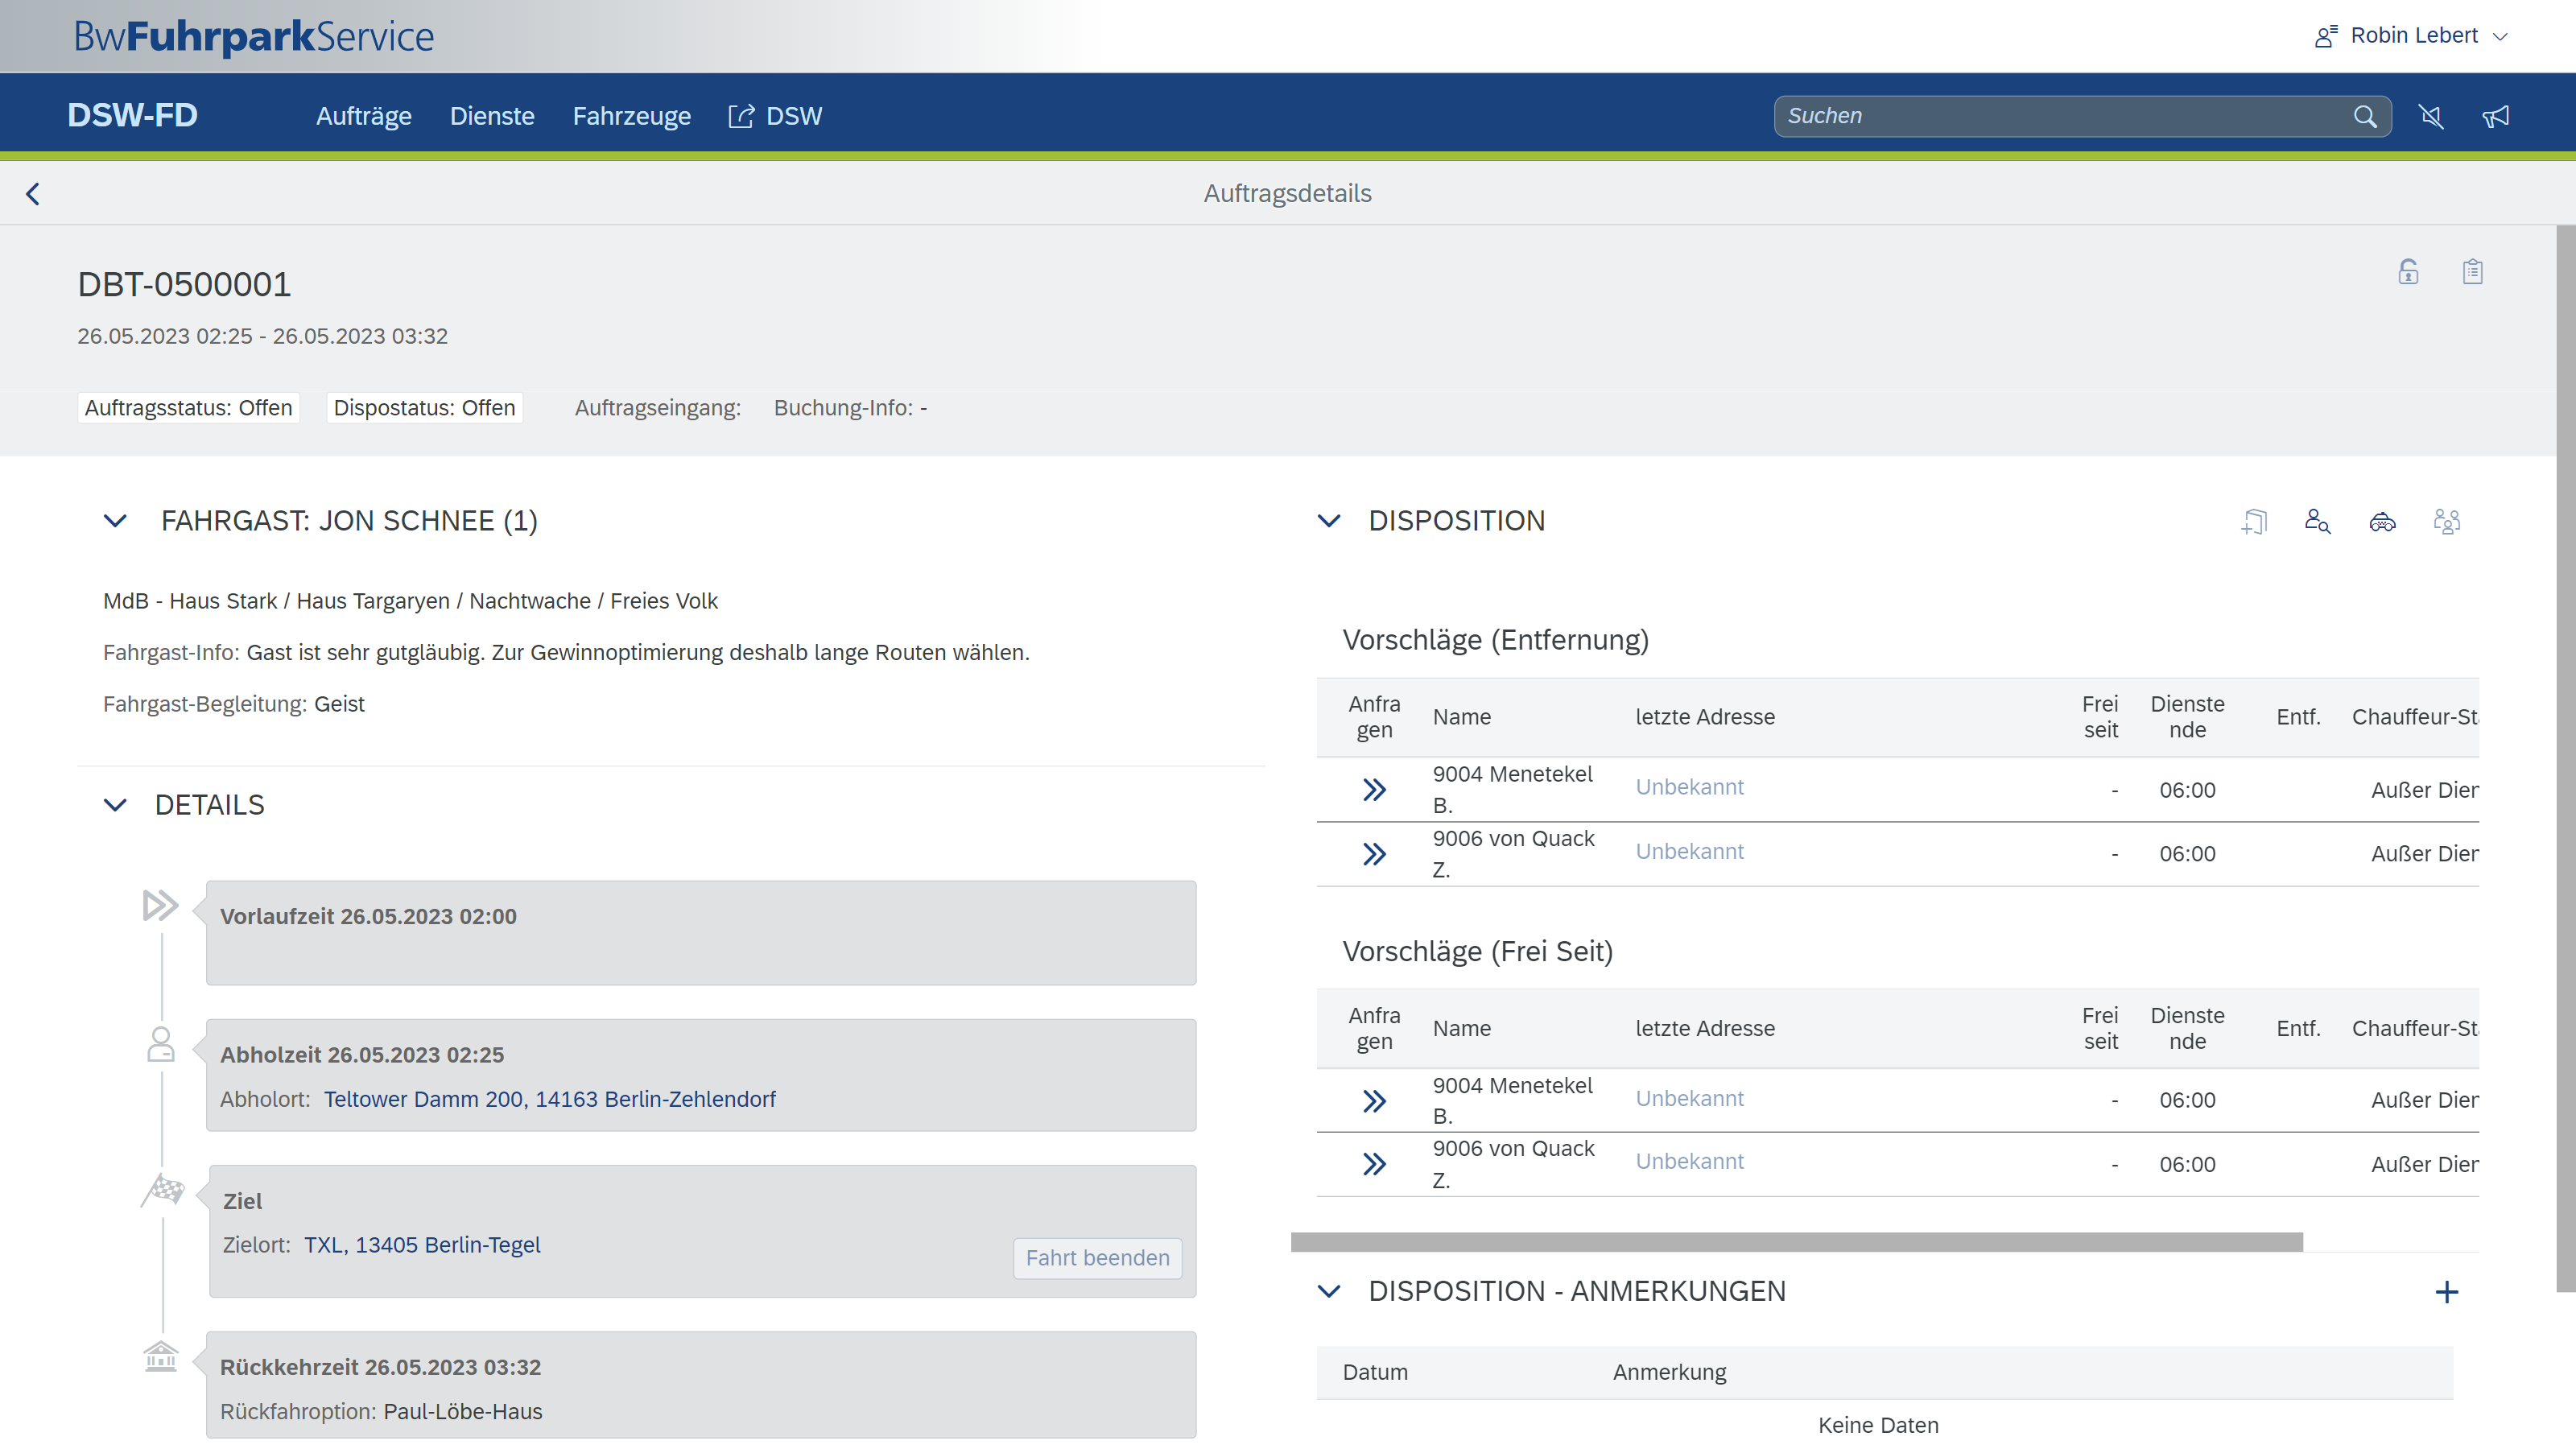
\includegraphics[width=\linewidth]{assets/current-auftrag-details}
    \caption{Chauffeur job details view in current implementation}
    \label{fig:current-details-auftrag}
\end{figure}


\subsection{Full Stack Implementation}

% \begin{itemize}
%     \item prisma 
%     \item easier Authentication
% \end{itemize}
Our first approach was the full stack implementation. This implementation has to replace the UI5 frontend as well as the Spring backend (\Cref{fig:dswfd-architecture-fullstack}). To this end business logic, database communication and API's all have to be implemented in SvelteKit. We used Prisma\footnote{\url{https://www.prisma.io}} for object relational mapping to communicate with the database, because Prisma provides functionality to generate its data model from an existing database using introspection. This allowed us to save time on defining models.

\todo{I feel like this section needs more text}

\begin{figure}
    \centering
    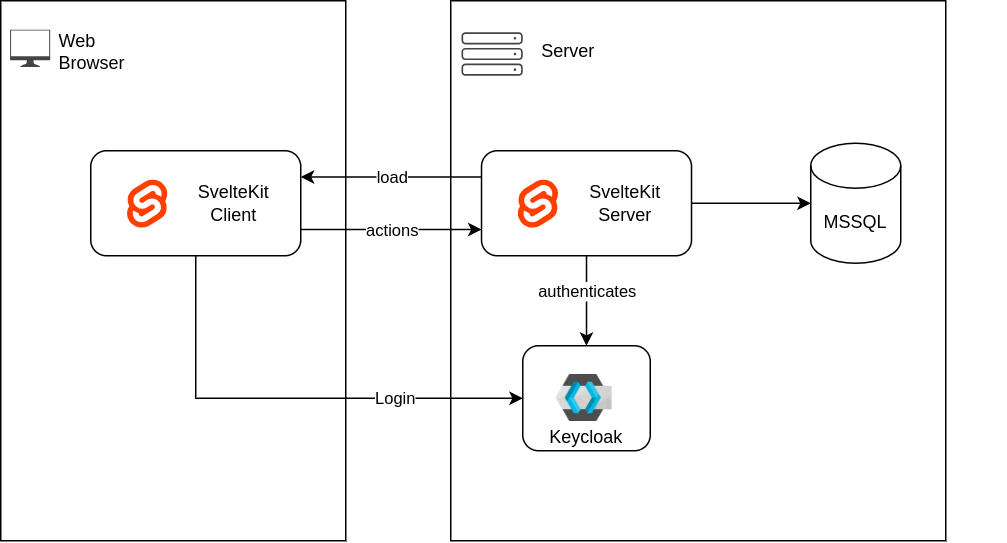
\includegraphics[width=.8\linewidth]{assets/dswfd-architecture-fullstack}
    \caption{Architecture overview of the implementation using SvelteKit as a full stack framework}
    \label{fig:dswfd-architecture-fullstack}
\end{figure}

\subsection{Frontend Implementation}

% \begin{itemize}
%     \item Experimented with direct communication to backend.
%     \item Using universal load functions
%     \item load on server during SSR,
%     \item then client takes over.
%     \item approach would make it possible to run app in SPA mode

%     \item Also tried to route all client requests through SvelteKit backend
%     \item easier because use of locales makes authentication simpler and no problems with custom fetch
%     \item enables usage of form actions, otherwise SvelteKit does not really provide any help with post requests.
% \end{itemize}

We also decided to explore an approach where SvelteKit is only used as a frontend. This approach provides more flexibility, as backend technology can be chosen individually. Communication to the backend is primarily handled using web API's. In our use case we decided to reuse the existing Java backend. The backend's REST API could be queried from SvelteKit. As REST APIs are something which can be called from frontend and backend, this approach can make use of SvelteKit's universal load functions (\Cref{sec:sveltekit-loading}). This means that the SvelteKit server is only used during SSR. After the browser has loaded the page, universal load functions are executed client-side and thus the client directs its requests directly to the backend instead of sending  a request to the SvelteKit server, which then requests the data, from the backend, overall saving one step of indirection. If loss of SSR is acceptable, this approach would also make it possible to run the application as an SPA, forgoing a dedicated SvelteKit server. This can be useful, as it allows for the SvelteKit application to be served as static files from a web directory or similar.

\begin{figure}[ht]
    \centering
    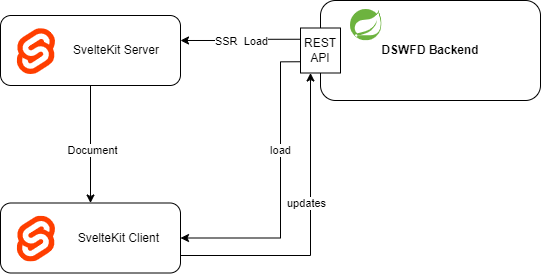
\includegraphics[width=.6\linewidth]{assets/fe-only-client-takes-over}
    \caption{Architecture overview of the implementation using SvelteKit only for the frontend}
    \label{fig:dswfd-architecture-fe-only}
\end{figure}

\subsubsection{redirect through server}

To amend these issues we further experimented with an implementation where we only used server load functions and server actions. This implementation is very similar to the full stack implementation discussed earlier. But instead of implementing business logic and database access in the SvelteKit server sided code, the server side is primarily used as middleware that sends REST requests to the Java backend.

\begin{figure}[ht]
    \centering
    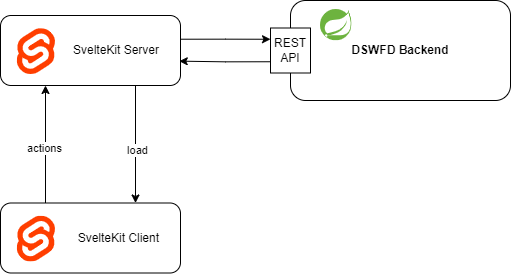
\includegraphics[width=.6\linewidth]{assets/fe-only-all-server}
    \caption{Architecture overview of the implementation using SvelteKit only as a frontend}
    \label{fig:dswfd-architecture-fe-through-server}
\end{figure}

This approach has multiple advantages. It uses much of the built-in functionality of SvelteKit, applications can be progressively enhanced, the client requires fewer dependencies, because functionality such as parsing and validating form data can be handled server side. Furthermore, authentication is simplified, as only the backend needs to communicate with the API. And finally, the outlined problems with fetch in universal load functions is solved, because only the backend uses fetch.


\subsection{UI Considerations}
\label{sec:implementation-ui}

One of the clients requirements for the current implementation was that the frontend follows the SAP Fiori design guidelines. While not strictly necessary for our study, we decided to adhere to this requirement in our SvelteKit implementations. We hoped to gain insights into how SvelteKit behaves, when interacting with UI libraries. The current implementation uses UI5 which has SAP Fiori components built into the framework itself. As it is not possible to use these components outside the framework, we had to use alternatives.   

We first tried to use UI5 Web Components\footnote{\url{https://sap.github.io/ui5-webcomponents/}}. These premade components promise to be a feature rich and framework-agnostic implementation of the Fiori Design Guidelines. In practice, we noticed multiple issues which made use consider alternative solutions. 

\todo{Finish section}

% Our first approach was to use SAP's UI5 Web components. Web components promise to be a framework-agnostic approach to UI components. But we encountered some problems early on:

% \begin{itemize}
%     \item For now, web components can not be server-side rendered. This is because web components rely on API's which only exist in the browser
%     \item Web Components also require JavaScript (at least until \cite{noauthor_declarative_2023})
%     \item Problems: Layout shifting, flash of unstyled content ("FOUC")
% \end{itemize}

\chapter{Evaluation}

\section{Empirical Data}

\subsection{Performance}

\subsection{Bundle Size}

Smaller, but no data yet...

\subsection{Something else}

\begin{itemize}
    \item SEO
    \item Community support
    \item DX
    \item ecosystem
    \item performance
\end{itemize}


\section{Experience}

\subsection{Cases where Svelte is great}

\begin{itemize}
    \item Concise / Intuitive Syntax
    \item reduction of client-server waterfalls
    \item SPA/SSR/SSG with single framework
    \item clear data flow (load function $\rightarrow$ svelte, svelte $\rightarrow$ action)
\end{itemize}

\subsection{Cases where Svelte is bad}

\begin{itemize}
    \item Centralized load function (compared to RSC's, load where needed)
    \item Things Which require node.js server (e.g. cron, websockets)
    \item Big data sets, which need to be shared between routes (virtuelle-fabrik)
    \item Style is scoped per default, thus it is annoying to pass classes to child component (improved with tailwind, because everything is global)
    \item Differences between client renderer and server renderer
    \item No best practices yet
    \item Problems with Svelte's Custom fetch
\end{itemize}




\chapter{Conclusion}
\label{ch:conclusion}

\todo{Write something}

\appendix
% hier Anhänge einbinden
\input{chapters/sources}

\backmatter
% \nocite{Knappen2009}
% \nocite{Mittelbach2005}
% \nocite{Schlosser2014}
% \nocite{Sturm2012}
% \nocite{Voss2010}

\printbibliography

\clearpage
\thispagestyle{empty}

Name: \fullname \hfill Matrikelnummer: \matnr \vspace{2cm}

\minisec{Erklärung}

Ich erkläre, dass ich die Arbeit selbständig verfasst und keine anderen als die angegebenen Quellen und Hilfsmittel verwendet habe.\vspace{2cm}

Ulm, den \dotfill

\hspace{10cm} {\footnotesize \fullname}
\end{document}
